\documentclass[12pt,fleqn,a4paper]{article}

\usepackage{latexsym}
\usepackage{url}
\usepackage{xspace}
\usepackage{epsfig}
\usepackage{psfrag}
\usepackage{a4wide}
\usepackage{marvosym}
\usepackage{amsmath,amsfonts,amssymb,amsthm,latexsym}
\usepackage{graphics,graphicx,color,subfigure}
\usepackage{fancyhdr}
\usepackage[english]{babel}
\usepackage[latin1]{inputenc}
\usepackage{listings}
\usepackage{comment}

\textheight 680pt
\textwidth 460pt
\topmargin -40pt
\oddsidemargin 5pt
\evensidemargin 5pt
\parindent 0pt

\pagestyle{fancyplain} \setlength{\headheight}{16pt}
\renewcommand{\sectionmark}[1]{\markright{\thesection\ #1}}
\lhead[\fancyplain{}{\thepage}]
    {\fancyplain{}{\rightmark}}
\rhead[\fancyplain{}{\leftmark}]
    {\fancyplain{}{\thepage}}
\cfoot{}
\renewcommand{\thesection}{\arabic{section}}
\renewcommand{\thesubsection}{\arabic{section}.\arabic{subsection}}


\begin{document}
\begin{titlepage}%Institution
\vspace{2cm}
\centerline{
\large{Department of Computer Sciences}}
\vspace{0.2cm}
\centerline{\large{University of Salzburg}}%Title with one or two Lines(More if wanted)
%\hline
\vspace{2cm}

\centerline{\large{PS Natural Computation}}
\centerline{SS 15/16}
\vspace{1cm}

\centerline{\Large{\bf{Evolution of a Poker Player Using Genetic Programming}} }%Type of the Document
\vspace{1cm}

\vspace{0.4cm}%Date
\centerline{\today}
\vspace{4.5cm}%Authors

%\hline
\vspace{0.2cm}
Project Members:\\
\centerline{Thomas Samy Dafir, 1331483, tdafir@cosy.sbg.ac.at}\\
\centerline{Laurentiu Vlad, 1423336, lvlad@cosy.sbg.ac.at}\\
\centerline{Dominik Baumgartner, 0920177, dbaumgart@cosy.sbg.ac.at}\\
\centerline{Sebastian Strumegger, 1420277, sstrumegg@cosy.sbg.ac.at}\\
\vspace {1cm}\\

Academic Supervisor: \\
\centerline{Helmut MAYER}
\centerline{helmut@cosy.sbg.ac.at}
\vspace{1.5cm}\\
Correspondence to: \\
\centerline{Universit\"{a}t Salzburg} \\
\centerline{Fachbereich Computerwissenschaften} \\
\centerline{Jakob--Haringer--Stra\ss e 2} \\
\centerline{A--5020 Salzburg} \\
\centerline{Austria}
\clearpage
\end{titlepage}

%Table of Content
\setcounter{page}{1}
\pagenumbering{Roman} %I,II,III... in the TOC
\tableofcontents

\clearpage
\pagestyle{headings}
\pagenumbering{arabic}  %Better if TOC is variable (more than one page)
\setcounter{page}{1}
\pagenumbering{arabic}  %Better if TOC is variable (more than one page)
\setcounter{page}{1}

\abstract{
This project focuses on the evolution of a computer poker player by means of Genetic Programming. The initial population evolves through selection, mutation and crossover of their strategies represented as syntax trees. Evolution selects the best players of every generation based on their fitness value which corresponds to their won chips and hence the quality of their strategies. In the end the fittest player emerges.
The focus of this project lies on making more information available to each computer player in order to let them make better poker moves which ultimately leads to improved evolved players emerging from the evolutionary process. This is done through determining which information is relevant and making it available to be used in a players strategy. An important objective is not to improve strategies ourselves but rather provide information to computer players and let evolution run its course to complete this task.
Furthermore, fine tuning of evolutionary parameters like mutation rate, population size and number of generations is conducted to achieve the best possible result.
}

\section{Introduction}
In the following article we explain our way from the general rules of a poker game to the final results of our project. \\
The goal is to improve an existing genetic programming poker player by providing additional information about the game.
To achieve this, basic knowledge about evolution and genetic programming is needed. We explain everything needed to know, so that anyone reading this article can follow our steps. \\
For the implementation of a genetic programming poker player we used existing frameworkss, so the main focus does lie in experimenting and not in implementing.
Hence this article does not contain any actual code examples, at most pseude code.
We start by explaining the poker game and its rules, where in this project only Texas Hold'em Poker is played.
Then we show some important ideas that describe genetic programming and give a short overview about the frameworks used, namely GPoker and JEvolution.
Finally the experiment setups and results are show and summarized.

\newpage
\section{Poker - The Game}
Poker is a gambling card game. The card pack consists of fiftytwo cards, which are divided into four colors: Hearts, Spades, Diamond and Clubs. Each of these four colors posseses nine cards which are numerated ascending from two to ten and four face cards: the Jack, the Queen, the King and the Ace.
\begin{figure}[!h]
	\begin{center}
		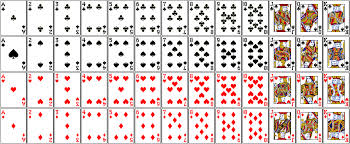
\includegraphics[width=10cm, height=5cm]{cards.jpg}
		\caption{Card Pack}
	\end{center}
\end{figure}
\\
To play the game a minimum of two players is needed. In this case it is called "Heads up". Every player starts with a specific amount of Chips, which are the currency in the game. Every turn each player has to bet an according amount of Chips. The options for betting are "check", "call", "raise" and "fold". If there are currently no bets, a player can check, which is equivalent to bet zero. If there are already some bets a player can call, which means to match the current bet made by an other player. Raise means to increase the size of the current bet and fold means to discard the cards and leave the round. This bets are collected in the so called "Pot". In the end the players have five random cards from the card pack on their hands. The winner of a round is the player with the best combination of cards in his hand and wins the pot.

\subsection{Card Combinations}
There are several card combinations which are ordered hierachically:
\begin{itemize}
	\item \textbf{High Card:} This is the lowest possible combination. In this case only the highest card value counts.
	\item \textbf{One Pair:} This is the next higher combination. Here the player posseses two cards of the same number or figure.
	\item \textbf{Two Pairs:} Same as before, but only with two times a pair.
	\item \textbf{Three of a Kind:} Here the player has three cards of the same number or figure on his hand.
	\item \textbf{Straight:} For this combination, the player must have five cards in ascending order on his hand. The color of the cards doesn't matter. 
	\item \textbf{Flush:} To achieve this combination the player must have five cards of the same color.
	\item \textbf{Full House:} The Full House consists of one pair, followed by three of a kind.
	\item \textbf{Four of a Kind:} Here the player has four cards of the same number or figure on his hand.
	\item \textbf{Straight Flush:} For the Straight Flush the player must have a Straight and all cards must be in the same color.
	\item \textbf{Royal Flush:} The last and highest combination is the Royal Flush. Therefore the player must have a Straight Flush with the five highest card values: ten, jack, queen, king and ace. 
\end{itemize}
	\begin{figure}[!h]
		\begin{center}
			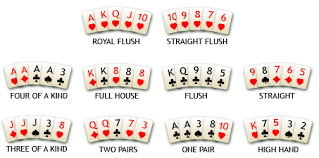
\includegraphics{combinations.png}
			\caption{Possible combination of cards}
		\end{center}
	\end{figure}
	
\subsection{Variants of Poker}
There are many different variants to play Poker. The most popular poker variants which are played in casinos and poker rooms can be divided into the following groups:
\begin{itemize}
	\item \textbf{Draw Poker:} In this type of games the players are dealt a complete hand, this means all five cards, hidden. Then the players can improve their hand by replacing cards.
	\item \textbf{Stud Poker:} Games in which the players recieve a specific amount of face-up cards and face-down cards in multiple betting rounds.
	\item \textbf{Community card Poker:} The players recieve a incomplete hand, which means not all five cards. This hand is then combined with the community cards which are face-up and can be used by each player.
\end{itemize}

\subsection{Texas Hold'em Poker}
This is a community card gametype. For this game two face-down cards are dealt to each player. This are the hand cards.
Then five community cards are dealt in three stages. The first betting stage is the "Flop". The Flop consists of three cards. The next stage is the "Turn", now one more community card is dealt. The last stage is the "River", where the final community card is dealt. Now each player has to seek out the best five card combinations by using his two hand cards and three community cards. Like in all other Poker games, the players have the options to check, call, raise or fold in each betting round.

\newpage


\section{Genetic Programming}
\label{sec:genprog}
Genetic Programming is an evolutionary method that tries to solve a complex problem by evolution.
After defining the problem, an initial population is created which is going to be evolved.
Further a fitness function is needed, that determines how fit an individual is for the problem.
This can be for example the amount of won poker chips in a game.
Individuals with a high fitness value are considered fitter and are candidates for evolution, which are then evolved by mutation or crossover.
We will further use the example of a Genetic Programming poker player with a tree representation.

\subsection{Program Tree}
A GP Player is represented by a program tree. More precisely, the poker player's strategy is represented by this tree.\\
This means, that each player's tree has a root node and zero or more child nodes, where nodes with children are called functions and leaf nodes are called terminals.\\
From the very beginning there is a fixed set of functions and terminals available.
At first, a population of GP Players with random nodes are created which play a predetermined number of games.
In each generation there is a probability for every player to get its tree changed by mutation or crossover.


\subsubsection{Functions}
\label{sssec:functions}
Functions play the most important role in a GP Player's strategy, since functions are the decision-makers.\\
They can have one or more child nodes and a specific return type. Further all nodes (except the root)  need to have a parent node.
Child nodes can either be terminals or functions. It is vital that the child nodes return the very type the function expects.\\
As an example we could define a lower-than function that expects floating point values from both children and returns a boolean value to it's parent node.

\subsubsection{Terminals}
Terminals are the leaf nodes in a player's tree. They cannot have child nodes but return a certain type themselves.\\
This does not necessarily mean that a terminal's value has to be static. They can have dynamic values like "pot size" or "higher hand card".

\subsubsection{Root}
The root node is a special function, since it does not have any parent nodes.\\
For proper evaluation of the player's tree it needs to be rooted, so we can start making further decisions at one point.
For GPoker we need to have a root node that always returns a poker move which is returned to the game.\\

\newpage

\subsubsection{Example}
\begin{figure}[!ht]
\begin{center}
	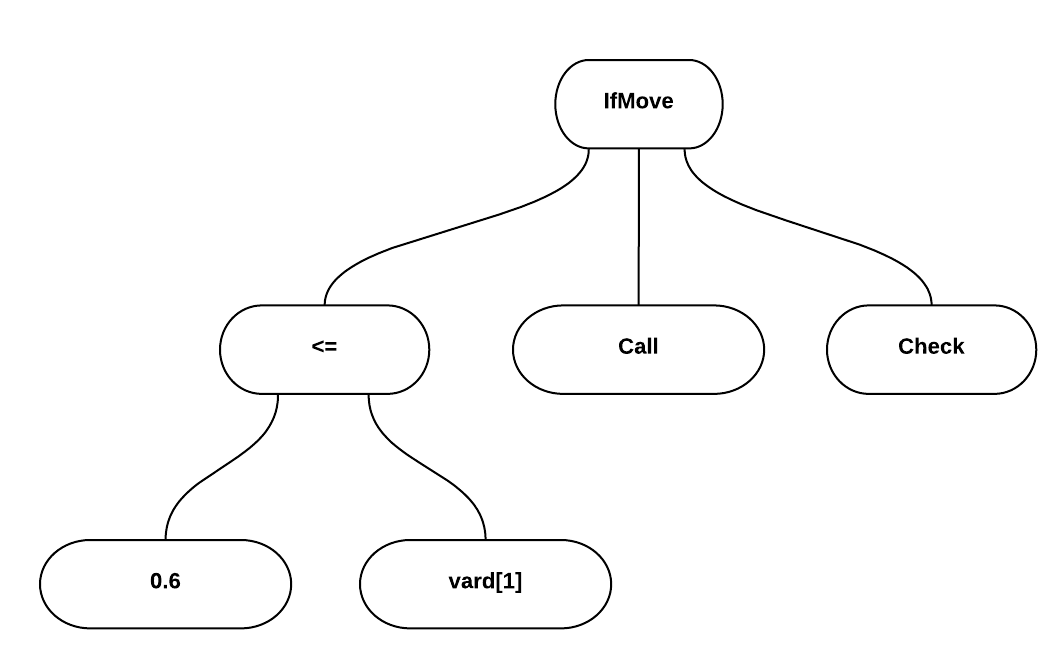
\includegraphics[width=0.8\textwidth]{tree1.png}
\caption{Example Tree of a GP poker player}
\end{center}
\end{figure}
This very simple tree represents the following strategy:
~\\
If 0.6 (Two to Ace normalized in 0 to 1) is less than or equal to the player's lower hand card, make a call.\\
Else: check. Note that checking can also mean folding, in case there has been a raise.

\subsection{Evolution}
\label{evolution}
There are two ways for evolution to change a tree, namely crossover and mutation.

\subsubsection{Crossover}
Crossover takes two individual players and swaps random subtrees.
Of course both subtrees need to have the same return type.
This method is more common, since good players that were not sorted out by evolution usually have good subtrees.
So the the well-playing trees are not completely destroyed by the process of evolution, but there is much room for new combinations.

\begin{figure}
\begin{center}
	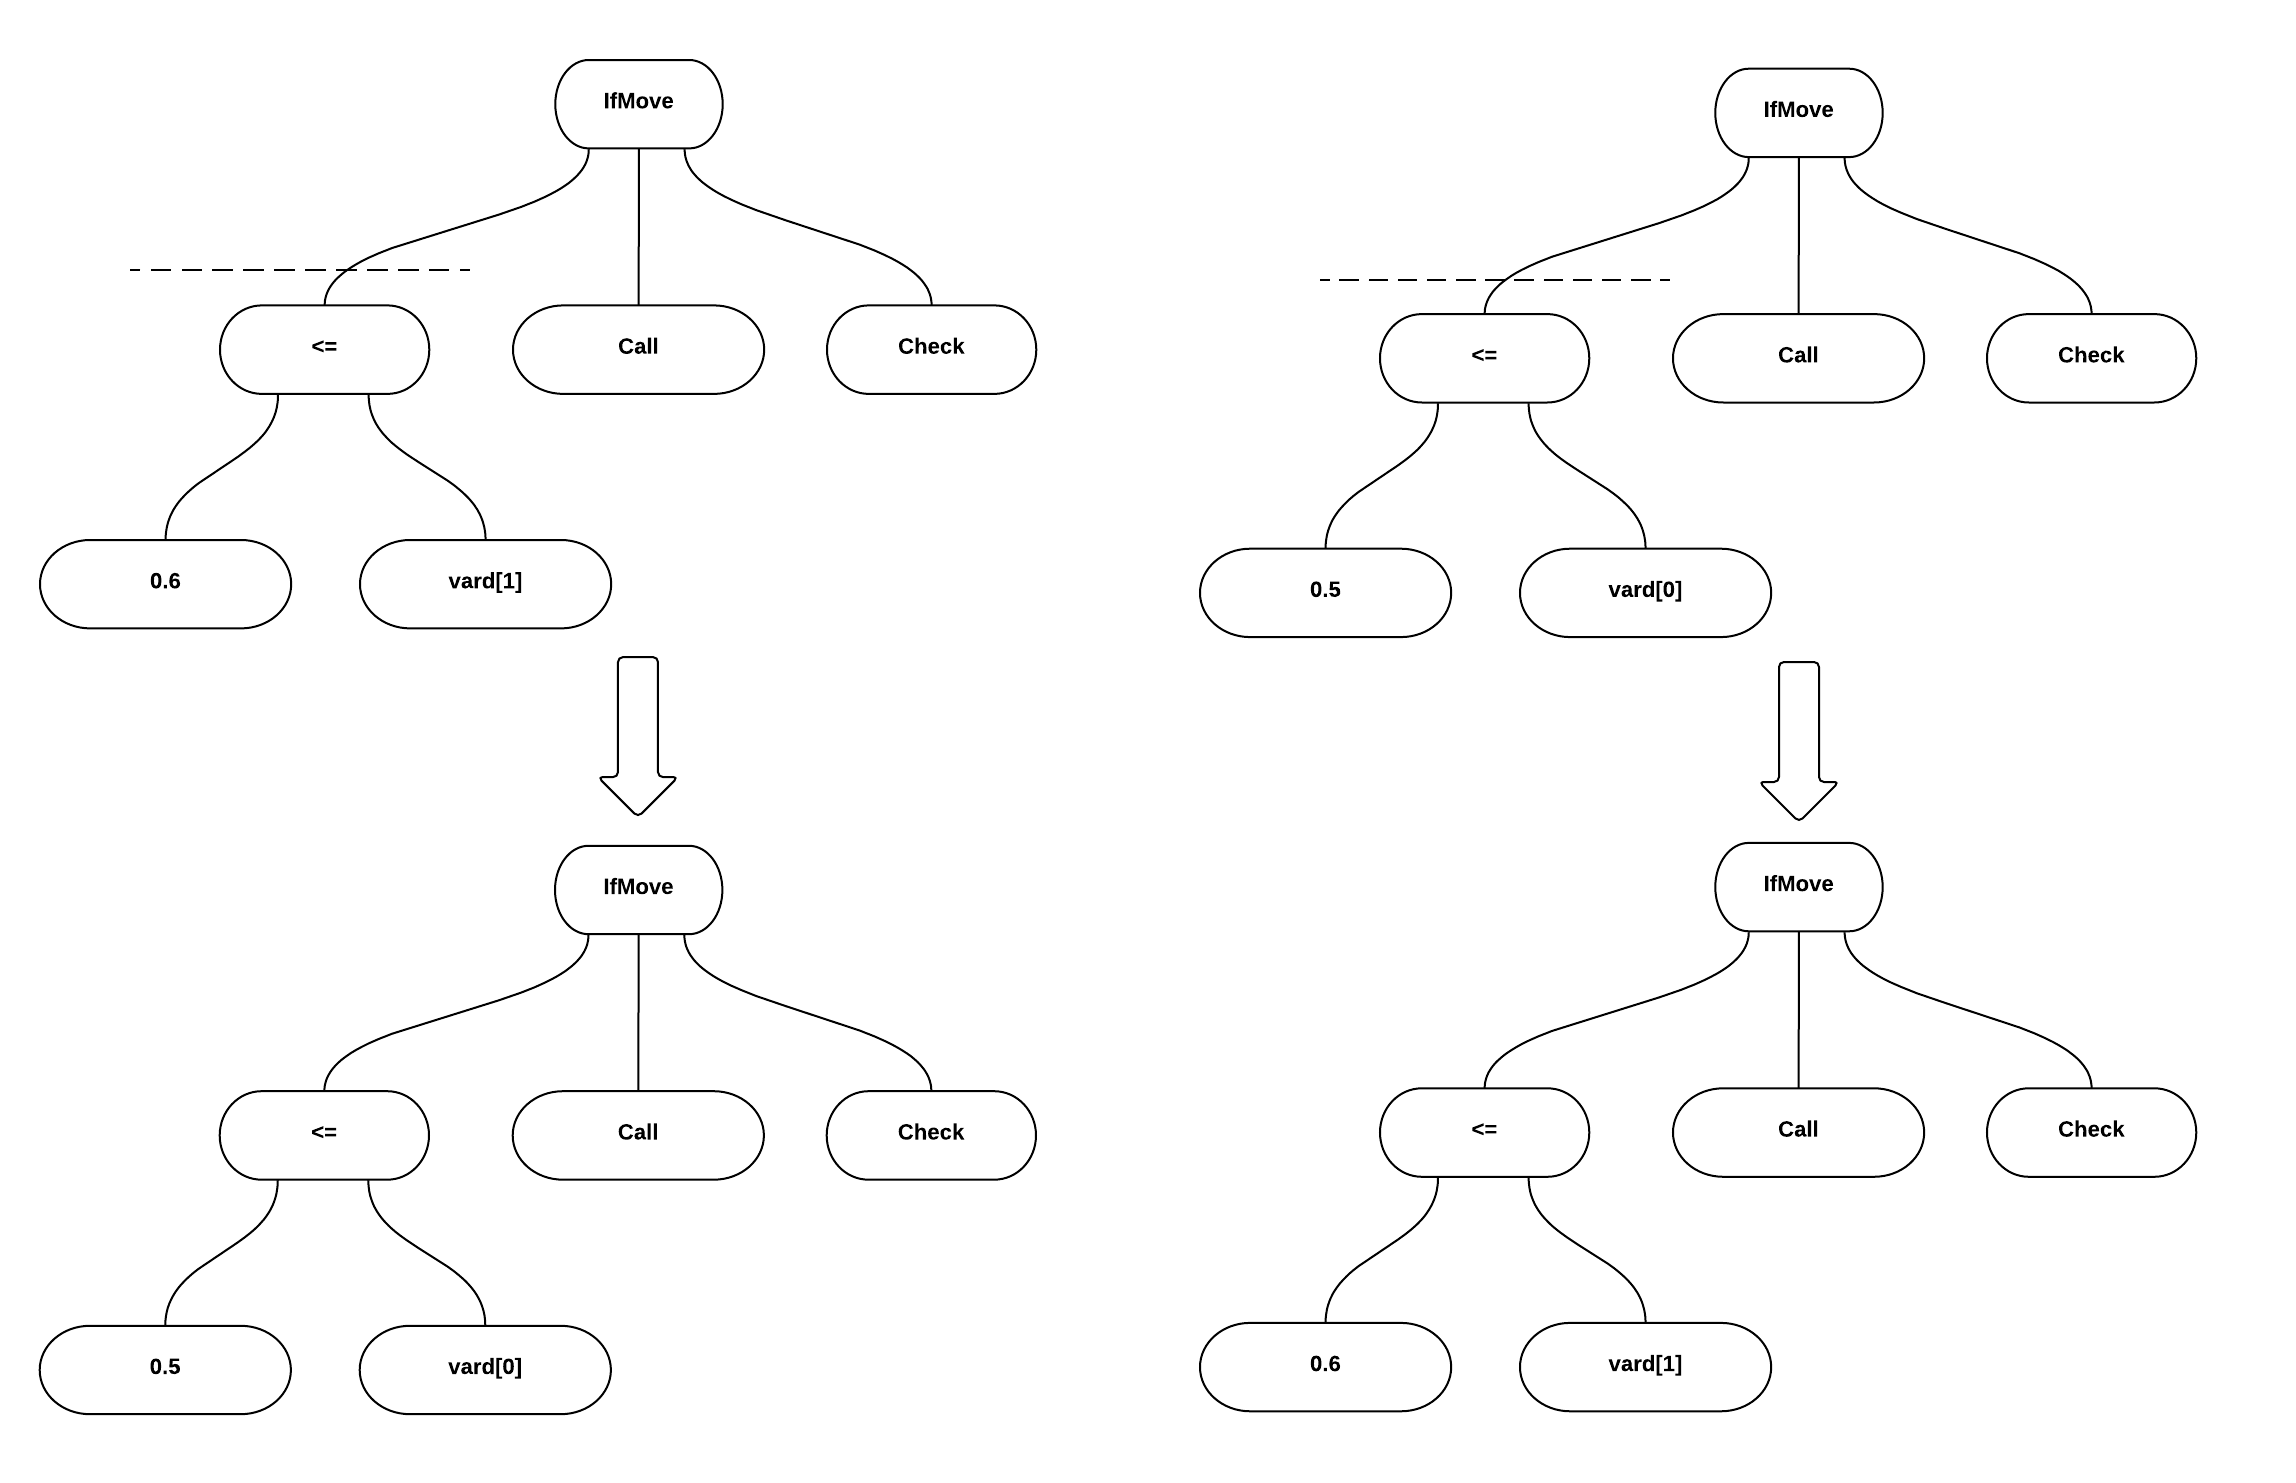
\includegraphics[width=1.0\textwidth]{tree_crossover.png}
\caption{Example for crossover}
\end{center}
\end{figure}

\subsubsection{Mutation}
In contrast to crossover, mutation does not require two individual trees to operate.
Either a single node is chosen at random and changed to some other random node with the same return type,
or a randomly chosen subtree is modified.

\begin{figure}
\begin{center}
	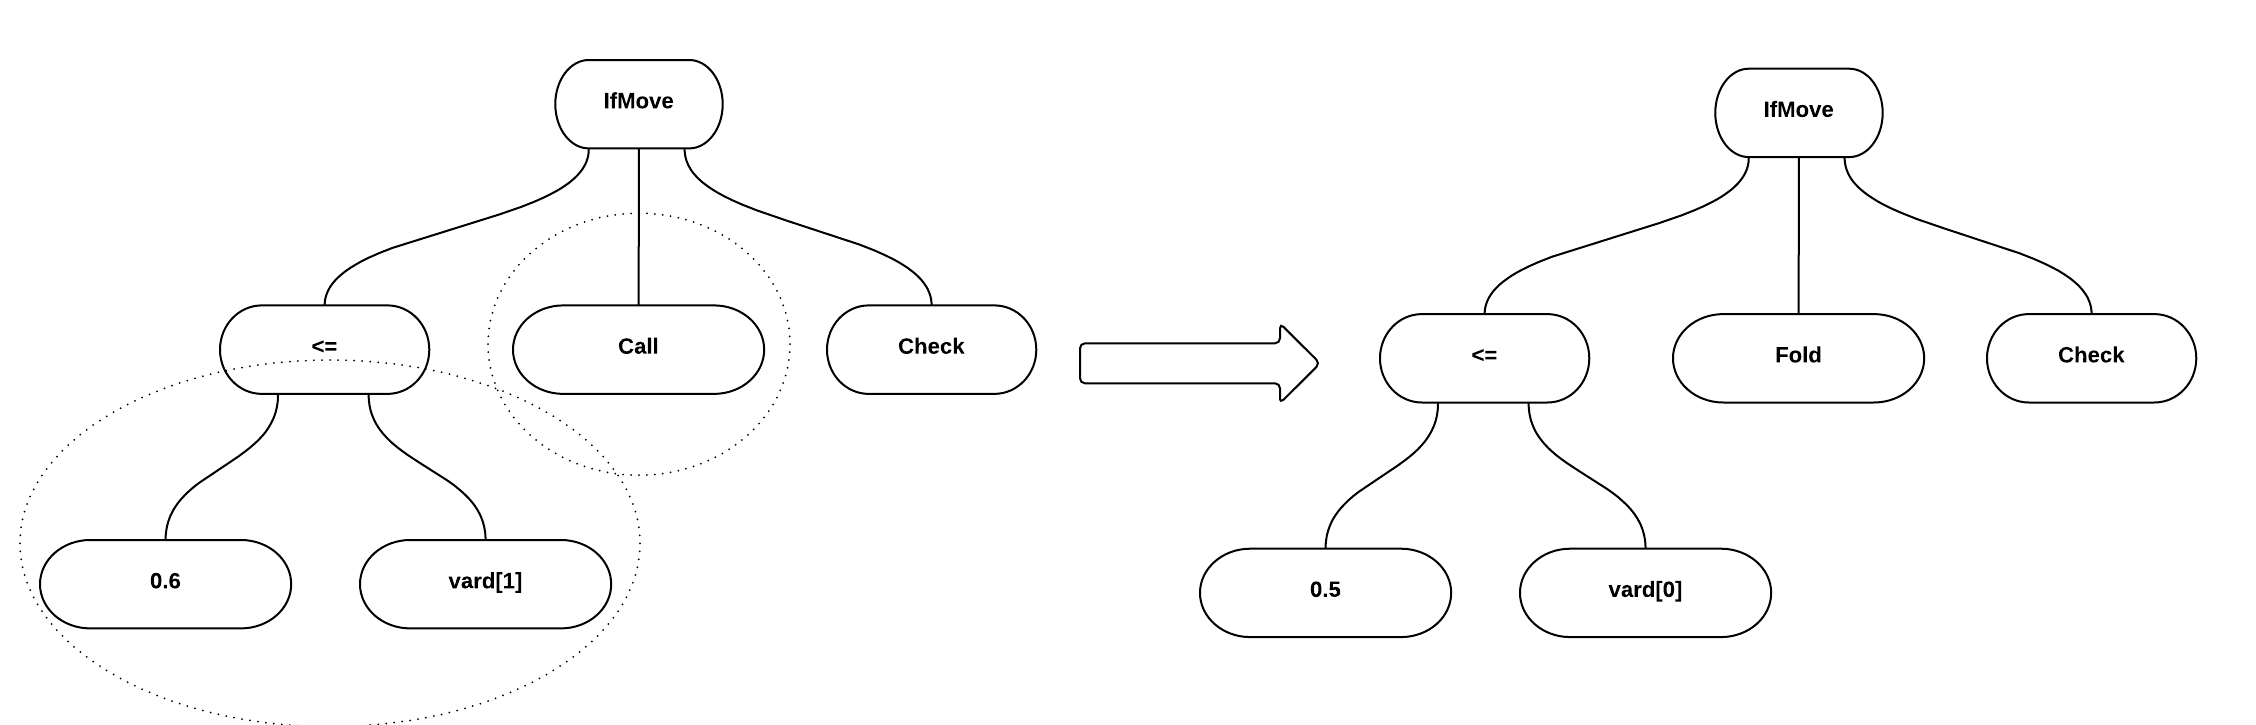
\includegraphics[width=1.0\textwidth]{tree_mutation.png}
\caption{Example for mutation}
\end{center}
\end{figure}
\newpage

\section{Frameworks}
\subsection{JEvolution}
JEvolution is a framework implementing several methods of evolutionary computing including Genetic Programming. JEvolution
conducts Genetic Programming as described in section \ref{sec:genprog}. It takes a node set and creates syntax trees. These
syntax trees are then evolved using selection, mutation and crossover. JEvolution selects trees with the highest fitness value which has to correspond to the ability of a player to "survive" in the surrounding environment.
In this application surviving means winning more chips and hence emerging as a winner in more games. Fitness calculation of a GPlayer is done by GPoker. 

\label{gpocker}
\subsection{GPoker}
GPoker is a poker-framework by Edgar Ebensberger \cite{GPoker}. GPoker implements a working no-limit no-rebuy Texas Hold'em poker setup. The implementation was done in Java. This object oriented approach made a design possible where aspects and components of a real poker game are represented directly by the class structure. These components include amongst others a dealer, players, strategies, cards and decks. GPoker allows the parameterization of many aspect of poker including the game-mode, big and small blinds as well as the involved players using a configuration file. There are preimplemented players including a check- and random-player as well as a player following a specific pattern and a human-player.
GPoker does not necessarily have to use Genetic Programming which is only invoked if an evolved player is participating in a game.
If this is the case GPoker invokes JEvolution which then evolves the player using the supplied node-set. The nodeset determines which information is available to the player as well as which actions the player is able to perform. Nodes are divides into terinals and functions. The following nodes were already implemented \cite{GPoker}:

\begin{itemize}
	\item ConstMove: represents one of 4 four poker moves: Raise, Call, Check, Fold. Results in another random
	move if mutated.
	\item ConstDouble: contains a constant double value ranging from 0.0 to 1.0.
	\item VarDouble: contains a variable double value ranging from 0.0 to 1.0. Originally only used to representate
	cards where 0.0 represents a deuce and 1.0 an ace. After extension of the framework VarDouble is now also used to
	hold hand values and the current game stage.
	\item IfMove: checks a condition and executes the instructions in the left path if the condition is met otherwise the 
	right path gets excuted. Returns a one of the four poker moves.
	\item ConstBoolean: contains a constant boolean value ("true" or "false").
	\item LessEqualBoolean: a function node which compares the two double values of its child nodes and returns true in case of the left value being less or equal compared to the right value. Otherwise false is reutrned.
	\item MultDouble: a function node which returns the product of its child nodes (a double value).
\end{itemize}

\subsection{Interactions}
Interactions between the two mentioned frameworks (namely JEvolution and GPoker) are essential to achieve the evolution of a poker player through Genetic Programming. Evolution works as follows:
\label{sec:nodes}
\begin{enumerate}
	\item A game of poker is startet through GPoker which checks if a GPlayer is amongst the players.
	\item If this is the case JEvolution is invoked to create an initial population of players represented by syntax trees
	made up from the nodes defined in GPoker.
	\item The fitness of each player (syntax tree) is determined by letting them play games of poker. The fitness value is defined as the total amount of chips a player has won.
	\item Selection is conducted on the population by selecting the players with the highest fitness values which are ultimately those who won the most chips and played best.
	\item The new generation is then repopulated through mutation and crossover (more information in section \ref{sec:genprog}).
	\item Then the whole circle is repeated using this new generation.
	\item This is repeated until the defined amount of generations has been reached and ultimately the best player is selected.
\end{enumerate}

\section{Experiment Setup}
For this experiment, some nodes got altered and one new node got introduced to test weather this results in a improved (higher) fitness of the evolved poker players. However, a higher fitness does not always necessarily mean that a player is better than one with with a lower fitness (see \ref{fitness}) since poker is not a transitive game. That means that if player A beats player B and player B beats player C, than player A does not necessarily beat player C.\\
Two players, each with a different setup of nodes, evolved against the "PatternPlayer" and the "TestPlayer" in multiple runs.

\subsection{Alterations}
The following additions and alterations had been done to the fixed set of nodes explained in section \ref{sec:nodes}.\\\\
\underline{New:}\\
\textbf{IfDouble}: A function node (see \ref{sssec:functions}) that checks if a double value is present and executes the left path, otherwise the right path gets executed.\\\\
\underline{Changed:}\\
\textbf{RaiseMove}: A terminal node for raise which was previousely implemented in "ConstMove" (see \ref{gpocker}).\\
\textbf{NewConstMove}: The same terminal as "ConstMove" (see \ref{gpocker}) except that it now doesn't contain the raise anymore since raise is now a terminal on it's own.

\subsection{Node setup}
\label{ssec:nodesetup}
These are the node-setups for both players.\\
The player with Setup1 has the aforementioned new and altered nodes in his pool for evolution. The player with Setup2 has the the original function- and terminal-set without any additional alterations.\\

\begin{figure}[!ht]
	\begin{center}
	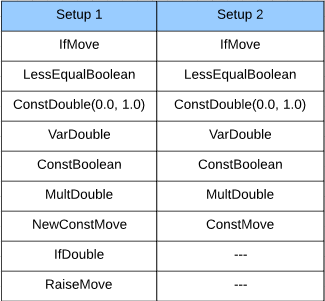
\includegraphics[width=.3\textwidth]{new_node_table.png}
	\caption{All functions and terminals used in the experiment devided in setups per player}
	\end{center}
\end{figure}	

The nodes:
\begin{itemize}
	\item LessEqualBoolean
	\item ConstDouble
	\item VarDouble
	\item ConstBoolean
	\item MultDouble 
\end{itemize}
are of no particular interest in this experiment. They were choosen because we want to test if wider range of nodes is beneficial for the evolution.

\subsection{Evolution against PatternPlayer}
\label{ssec:patternplayer}
The pattern player was choosen to evolve against, because it exhibits a play style that a new player to Texas Hold'em would have. Meaning that it plays defensively when his hand is not that great. It evaluates its hand (including community cards) and the hole cards. A normalized value is then calculated which in turn determines its next move.

\newpage

\subsection{Evolution against TestPlayer}
\label{ssec:testplayer}
One test player was choosen from previously evolved players which plays as follows.\\

\underline{Pseudocode:}\\

\textbf{if} highest card \textless \hspace*{0.5em}JACK \\
\hspace*{3em}\textbf{if} current bet for a call \textless \hspace*{0.5em}9 \\
\hspace*{3.9em} \textbf{return} CALL \\
\hspace*{2.5em} \textbf{else} \\
\hspace*{3.9em} \textbf{return} CHECK \\
\hspace*{1.5em} \textbf{else}  \\
\hspace*{3em} \textbf{return} RAISE(0.9849 * pot size) \\

\subsection{Fitness and fitness evaluation}
\label{fitness}
The fitness of a player is usually calculated via a fitness function which determines its performance or quality in the given environment. In the context of this project, the fitness is represented by the amount of chips a player had won.

\subsection{Selection and selection method}
\label{selection}
Some of the players of a given generation, are being selected in order to produce new player for the next generation. The selection method we chose is called "Tournament Selection" where the players with the highest fitness value of a parent population are picked in order to produce a new generation of players. The reason behind the concept of choosing the ones with the highest fitness is that they are more likely to produce new players that are "good" players (the ones achieving high fitness scores). 

\subsection{Doyle's Game}
\label{doyle}
Doyle's Game is a variant of no-limit Texas Hold'em and is being used in this experiment. In this variant of the game, each player can make an "all-in" bet, but the players stack size (the amount of chips a player has before making any bet, blinds included) are reset to some default size/amount after each hand. The won or lost chips of every player is stored separately for each one and does not affect the starting chips of the following games.\\\\
This approach prevents two problems:
\begin{itemize}
	\item a player going bankrupt during a game. Avoiding this is desirable since we want to evaluate each player against each opponent.
	\item a player having far more chips than his opponents since this can lead to all-in bets of unequal sizes between players.
\end{itemize}

\subsection{Input parameter}
\label{inputparameter}
For both experiments the parameters were chosen as follows: 
\begin{itemize}
	\item Game Mode: Doyle (see \ref{doyle})
	\item Test-Runs: 8 for each player/setup
	\item Generations: 10.000
	\item Population-Size: 100
	\item Rounds played per generation: 1000
	\item Mutation-Rate: 0.0369 (see \ref{evolution})
	\item Crossover-Rate: 1.0 (see \ref{evolution})
	\item Selection Method: Tournament selection (see \ref{selection})
	\item Chips/Player: 1000 
	\item Big blind: 10
\end{itemize} 
A generation of 10.000 seemed to be sufficient for an overall assessment of the fitness. In test runs using 20.000 generation it was noticed that
the player with the highest fitness would always emerge within the 10.000th generation.

\section{Example player with setup 1}
The figure below shows how a player might look like using the altered node setup (setup 1). See \ref{ssec:nodesetup}.
\begin{figure}[!ht]
	\begin{center}
		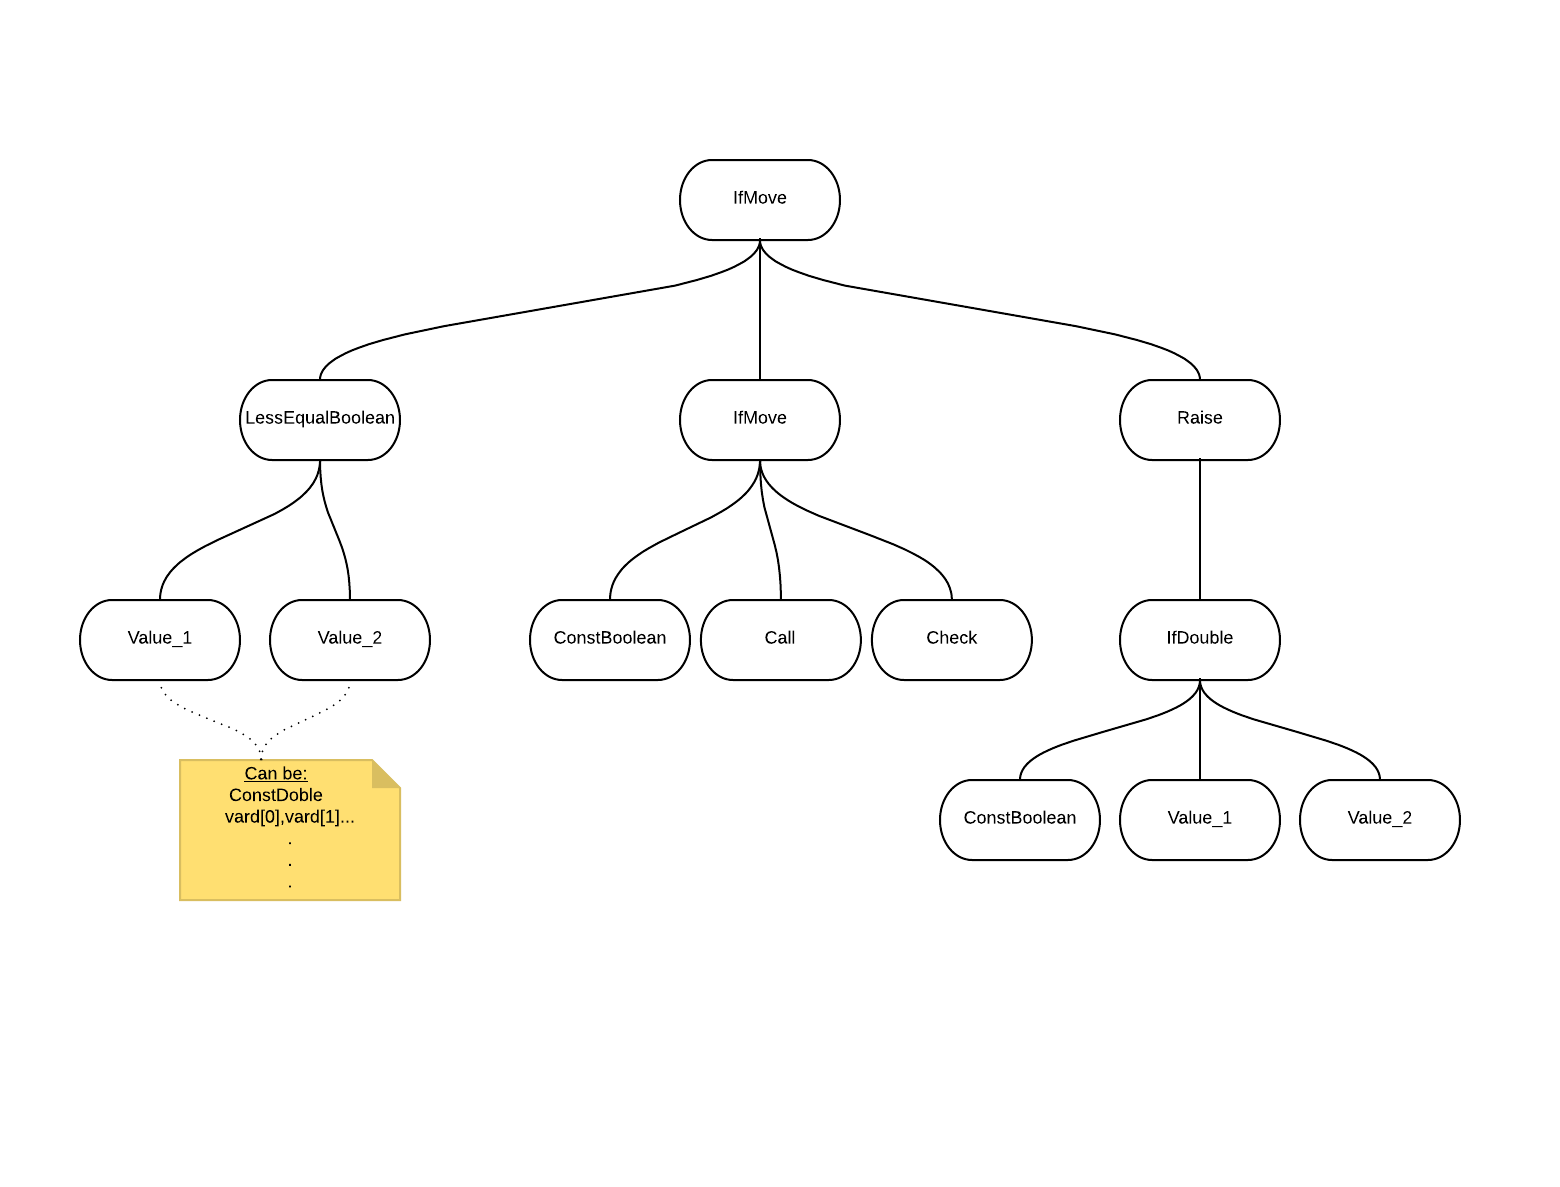
\includegraphics[width=0.95\textwidth]{NewRaise.png}
		\caption{Example tree of an evolved player with setup 1}
		\end{center}
		\end{figure}

\section{Experiment Results}
\label{sec:expres}
Each setup evolved against the "PatternPlayer" and the "TestPlayer"  
Please note that the values in the following diagrams are not plotted in the same order as they have been obtained from the test runs but are sorted in an ascending order!\\
Furthermore, 

\subsection{Evolution against PatternPlayer}
The evolution against the "PatternPlayer" resulted in a deterioration of the fitness of the player with "setup 1" compared to the player playing with "setup 2".\\
Further statistical test would bee needed in order to elucidate why the player with "setup 2" has an overall higher fitness.

\begin{figure}[!h]
	\begin{center}
	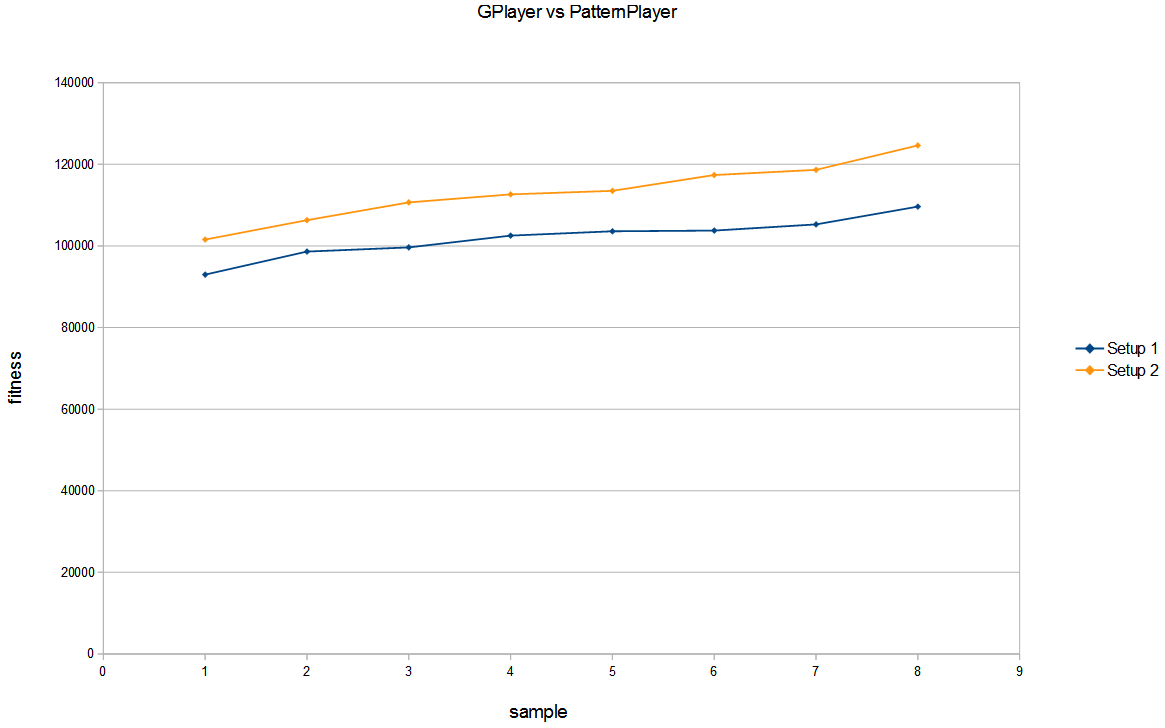
\includegraphics[width=.7\textwidth]{gp_vs_pp_new.png}
	\caption{The fitness results of both players playing against the "PatternPlayer" plotted in ascending order}
	\end{center}
\end{figure}

\newpage
\subsection{Evolution against TestPlayer}
Overall it is safe to say that the changes improved the performance against the TestPlayer. Although there can be some cases where the old player has a higher fitness than the new one. It was also notable that the overall fitness is cut down to approximately a third compared to the test runs against the PatternPlayer.

\begin{figure}[!h]
	\begin{center}
		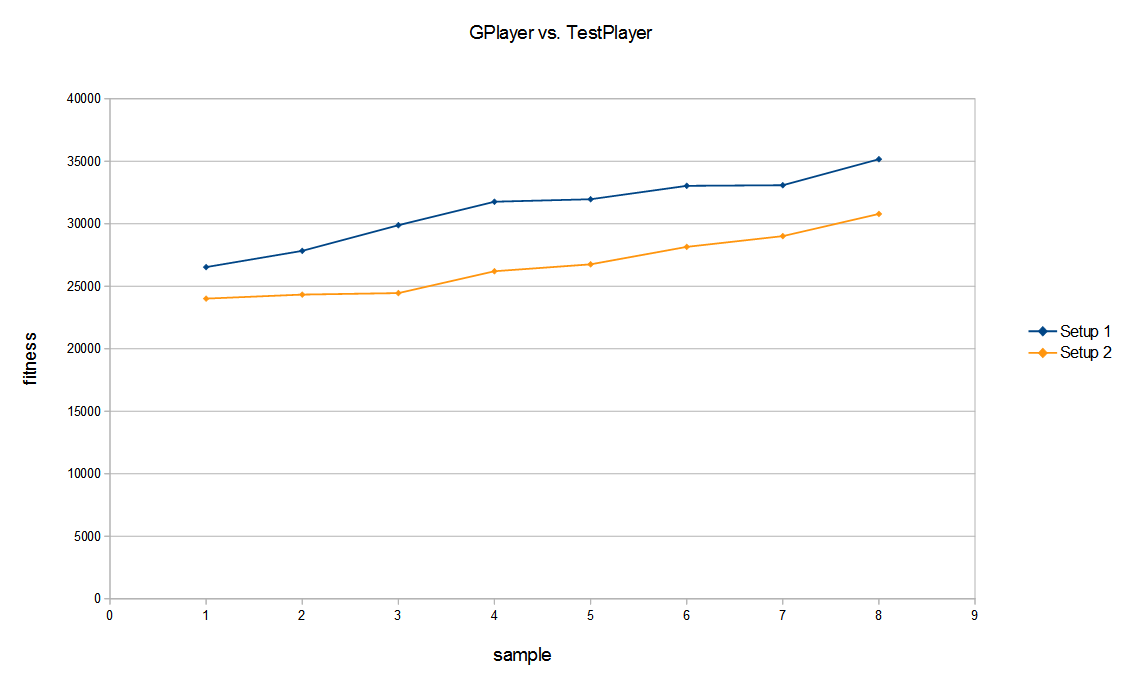
\includegraphics[width=.7\textwidth]{gp_vs_tp_new.png}
		\caption{The fitness results of both players playing against the "TestPlayer" plotted in ascending order}
	\end{center}
\end{figure}

\section{Summary}
The main objective of this project was to extend the already existing process of evolving a poker player through Genetic Programming. The focus lay on increasing the information available to the computer player by implementing new nodes to be used in the syntax tree defining a player's strategy. The main feature enabled by the newly implemented nodes is the added ability to evolve the value of a poker raise move (RaiseMove). Furthermore, there is a new node making it possible for the evolved player to work with different values (card values, stage value) depending on the current circumstances (IFDouble).
As the experiments in chapter \ref{sec:expres} have shown an overall increase in an evolved player's success can only be partly confirmed and is highly dependent on the opponent. Experiments where the computer player was evolved against a opponent following a certain fixed pattern showed no improvement. The second round of experiments was conducted against a sane player with a strategy a human might use. These results showed an increase in the evolved player's overall fitness of up to 30 percent compared to the original project state which is indeed a fairly significant improvement.

% links go here, NOT in references

\newpage
\section{Links}

\begin{itemize}
\item Project Page: \url{https://student.cosy.sbg.ac.at/~tdafir/nc/}
\item PS Page:
\url{http://www.cosy.sbg.ac.at/~helmut/Teaching/NaturalComputation/proseminar.html}

\end{itemize}

\nocite{*}
\bibliographystyle{ieeetr}
\bibliography{report_refs}		% .bib files here

\end{document}
